\chapter{Experiment Results and Evaluation}
\label{ch:evaluation}

\section{Evaluation Methodology and Field Contextualization}
Aetron was evaluated in two complementary tiers: (1)~\textbf{Smartphone Field Contextualization} carried forward from the pre-thesis evaluation~\cite{aetron2026prethesis} to verify real-world distance alignment against established commercial fitness apps and pre-measured urban routes; and (2)~\textbf{Reproducible Public-Dataset Benchmarking} executing both live runtime algorithms (EKF/AEKF, iOS light-free IOD, Model~C-Mobile, adapted MV-GLRT ZUPT, 6-second cadence, LOSO Renaudin stride, P03 reconstruction, and contiguous 2024 Compendium MET tables) and offline research comparators (sequential centroid-radius dwell clustering, linear-CV IGG-III/IAE, causal IMM/Zheng, and CAP-ALSTM + Python SHAP) on open public datasets with independent physical ground truth. Every offline experiment adheres strictly to an unbroken \textbf{Evidence Provenance Chain} summarized in Table~\ref{tab:evidence_chain}.

\begin{table}[htbp]
\centering
\caption{Complete Scientific Evidence Provenance Chain across All Evaluated Modules.}
\label{tab:evidence_chain}
\resizebox{\textwidth}{!}{
\begin{tabular}{@{}llllll@{}}
\toprule
\textbf{Module} & \textbf{Published Basis} & \textbf{Public Dataset} & \textbf{Ground Truth} & \textbf{Code / Benchmark Target} & \textbf{Primary Metrics} \\ \midrule
\textbf{1. Outdoor GNSS / EKF} & Groves~\cite{groves2013principles}; Sukhenko~\cite{sukhenko2025gnss}; & TU Wien RTK~\cite{tuwien2026gnss}; & Leica GS18 RTK; & \texttt{ExtendedKalmanFilter}; & Shared-mask RMSE, P95, \\
 & Rong Li~\cite{rongli2003survey}; Li~\cite{li2025trajectory} & SnapperGPS~2~\cite{beuchert2023snappergps} & u-blox ZED-F9P RTK & \texttt{run\_fixed\_alpha\_vs\_ekf.py} & Dist.\ Err., Cluster CI \\ \midrule
\textbf{2. Cross-Platform IOD} & Dastagir~\cite{dastagir2024deepiod}; Yoo~\cite{yoo2025seamless}; & Cambridge CIOD~\cite{bakirtzis2022ciod}; & Session-disjoint labels & \texttt{DeepIodNeuralClassifier}; & Acc, Macro-F1, In/Out Rec, \\
 & Ashraf~\cite{ashraf2018magio}; Zhu~\cite{zhu2019fast} & HAR-PMD~\cite{harpmd2025dataset} ($120$ subj.) & \& $46$ doorway transits & \texttt{IosMultiSensorIodClassifier} & Event F1, FT/hr, Delay \\ \midrule
\textbf{3. Step / MV-GLRT / Cad.} & Salvi~\cite{salvi2018oxford}; Xu~\cite{xu2022step}; & Oxford WPD; Xu G3; & Tally \& $60$\,fps video & \texttt{OxfordStepDetector}; & Count Acc, WAPE, False \\
 & Skog~\cite{skog2010zupt}; Brajdic~\cite{brajdic2013walk} & PedEval; OxWalk~\cite{oxwalk2022oxford} & ($119{,}572$ steps) & \texttt{StepMotionGate} / \texttt{Cadence} & Steps, MAE, Flutter, Lag \\ \midrule
\textbf{4. Adaptive Stride} & Renaudin~\cite{renaudin2012step}; & SLEDataset2~\cite{vezocnik2021sle} ($114$); & Optical MoCap \& & \texttt{ResearchStepLengthFallback} & Strict LOSO MAE (cm), \\
 & Fukuchi~\cite{fukuchi2017public} & Fukuchi RBDS ($84$ run) & Force-Plate Treadmill & \texttt{stride\_length\_benchmark\_test} & RMSE (cm), MAPE (\%) \\ \midrule
\textbf{5. Outage Reconst.} & Fritsch--Carlson~\cite{fritsch1980pchip}; & TU Wien ($10$ walks); & Held-out $5$\,s interior & \texttt{WorkoutSessionFinalizer} & Per-session \& Pooled \\
 & Czerwi{\'n}ski~\cite{czerwinski2026reconstruction} & SnapperGPS~2 ($12$ rides) & RTK coordinates & \texttt{replay\_tu\_wien\_p03\_closure.py} & RMSE, P95 (Display-Only) \\ \midrule
\textbf{6. Dwell \& Polyline} & Ester~\cite{ester1996dbscan}; Zheng~\cite{zheng2009mining}; & STAGA~\cite{spang2022staga} ($122{,}808$); & Mobility stop diary; & \texttt{GpsDbscanService}; & Stop Prec/F1, False Stops, \\
 & Herrmann~\cite{herrmann2024compendium} & $60$-min courtyard; $30{,}381$ pts & Stationary truth & \texttt{PolylineCompressionService} & Bytes Saved, MET Parity \\ \bottomrule
\end{tabular}
}
\end{table}

\section{Field Comparison with Commercial Reference Applications}
\label{sec:eval_commercial_field}
To contextualize Aetron against commercial applications in real outdoor conditions, six smartphones ran FITAPP, Goals-Fitness, Running by Adidas, Nike Run Club, Strava, and Aetron concurrently along the same urban park walking loop ($\approx 510$\,m, Route~B). Table~\ref{tab:commercial_route_b} and Figure~\ref{fig:route_b_comparison} show that Aetron recorded $0.52$\,km, squarely matching Strava ($0.52$\,km) within the $0.51$--$0.56$\,km commercial spread.

\begin{table}[htbp]
\centering
\caption{Recorded field metrics across six fitness applications on Route~B ($\approx 510$\,m urban walking loop; Strava summary screenshot omitted calories).}
\label{tab:commercial_route_b}
\resizebox{0.92\textwidth}{!}{
\begin{tabular}{@{}lcccc@{}}
\toprule
\textbf{Application} & \textbf{Duration} & \textbf{Distance (km)} & \textbf{Calories (kcal)} & \textbf{Avg Pace (min/km)} \\ \midrule
FITAPP & 08:06 & 0.51 & 44 & 15:58 \\
Goals-Fitness & 08:22 & 0.51 & 32 & 16:24 \\
Running (Adidas) & 07:57 & 0.56 & 32 & 14:08 \\
Nike Run Club & 08:09 & 0.51 & 28 & 15:47 \\
Strava & 08:16 & 0.52 & N/A & 15:54 \\
\textbf{Aetron (This Work)} & \textbf{08:21} & \textbf{0.52} & \textbf{34} & \textbf{16:03} \\ \bottomrule
\end{tabular}
}
\end{table}

\begin{figure}[htbp]
\centering
\begin{subfigure}[b]{0.31\textwidth}
    \centering
    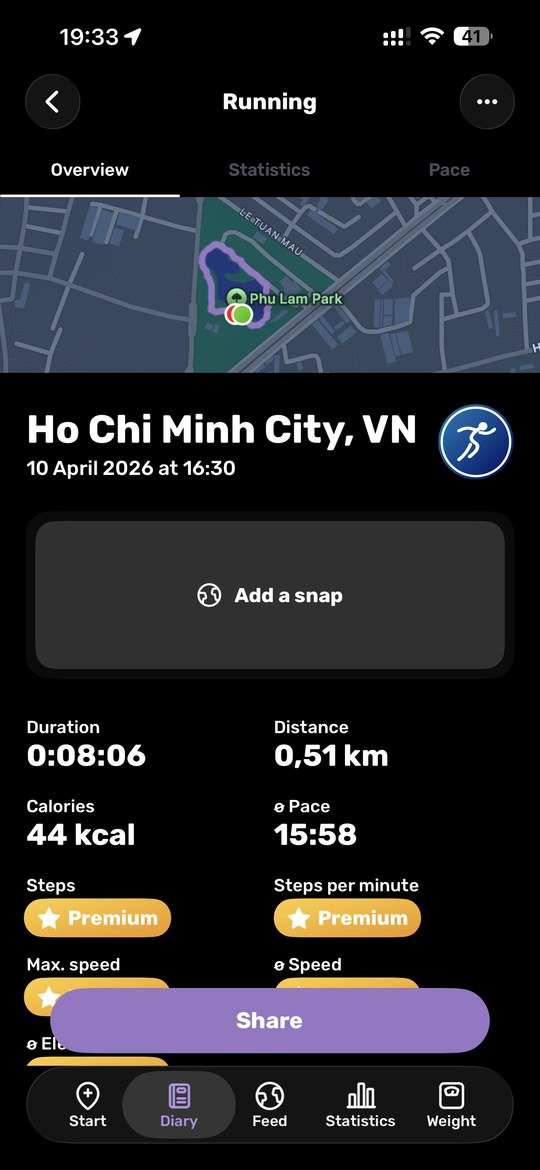
\includegraphics[height=5.2cm]{figures/cmp_fitapp.jpg}
    \caption{FITAPP ($0.51$\,km)}
\end{subfigure}\hfill
\begin{subfigure}[b]{0.31\textwidth}
    \centering
    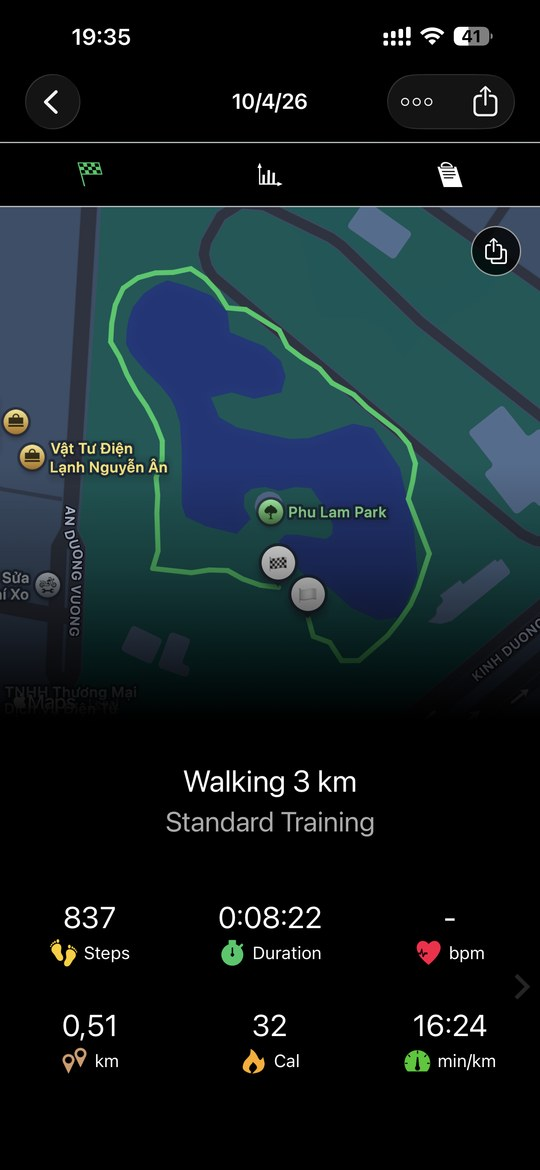
\includegraphics[height=5.2cm]{figures/cmp_goals.jpg}
    \caption{Goals-Fitness ($0.51$\,km)}
\end{subfigure}\hfill
\begin{subfigure}[b]{0.31\textwidth}
    \centering
    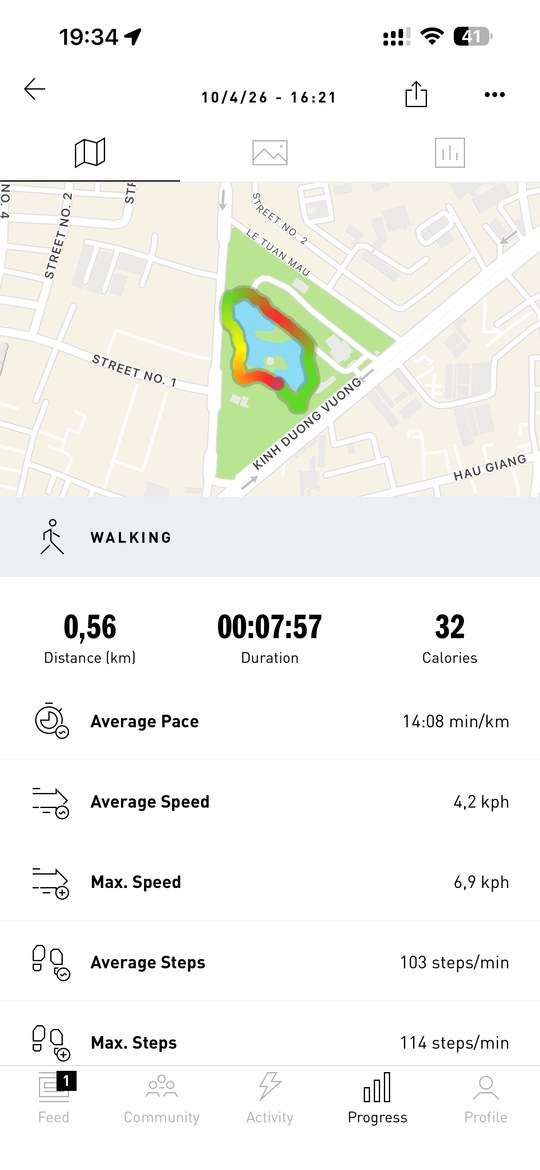
\includegraphics[height=5.2cm]{figures/cmp_adidas.jpg}
    \caption{Adidas Running ($0.56$\,km)}
\end{subfigure}\\[0.35cm]
\begin{subfigure}[b]{0.31\textwidth}
    \centering
    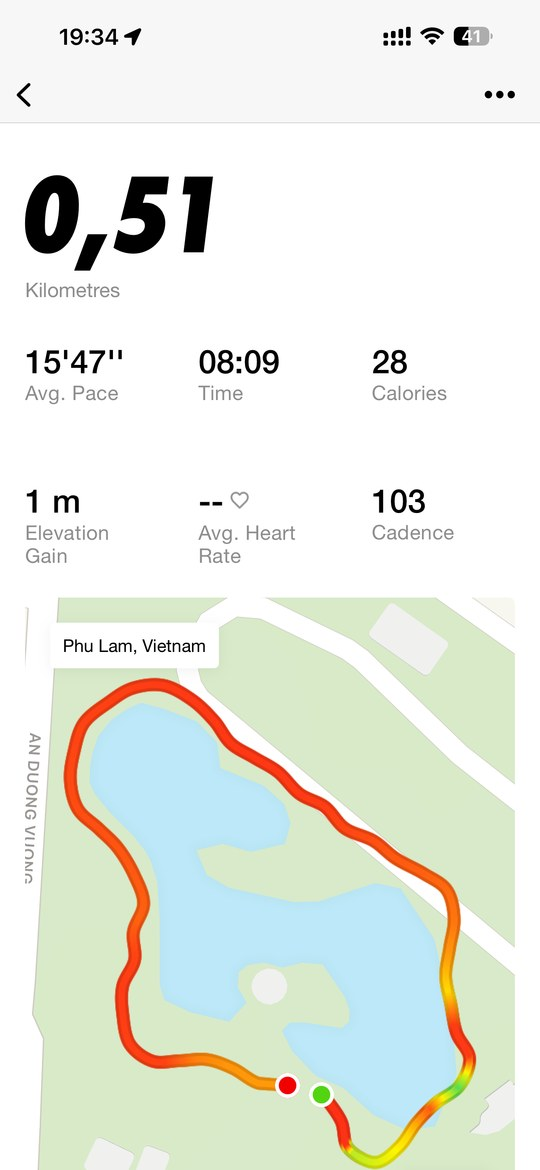
\includegraphics[height=5.2cm]{figures/cmp_nrc.jpg}
    \caption{Nike Run Club ($0.51$\,km)}
\end{subfigure}\hfill
\begin{subfigure}[b]{0.31\textwidth}
    \centering
    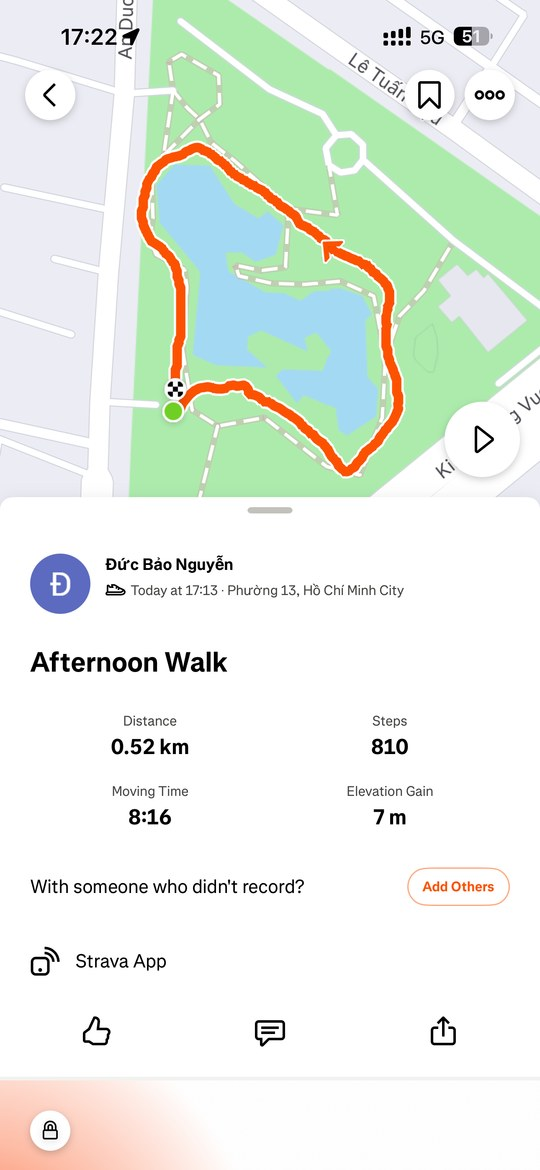
\includegraphics[height=5.2cm]{figures/cmp_strava.jpg}
    \caption{Strava ($0.52$\,km)}
\end{subfigure}\hfill
\begin{subfigure}[b]{0.31\textwidth}
    \centering
    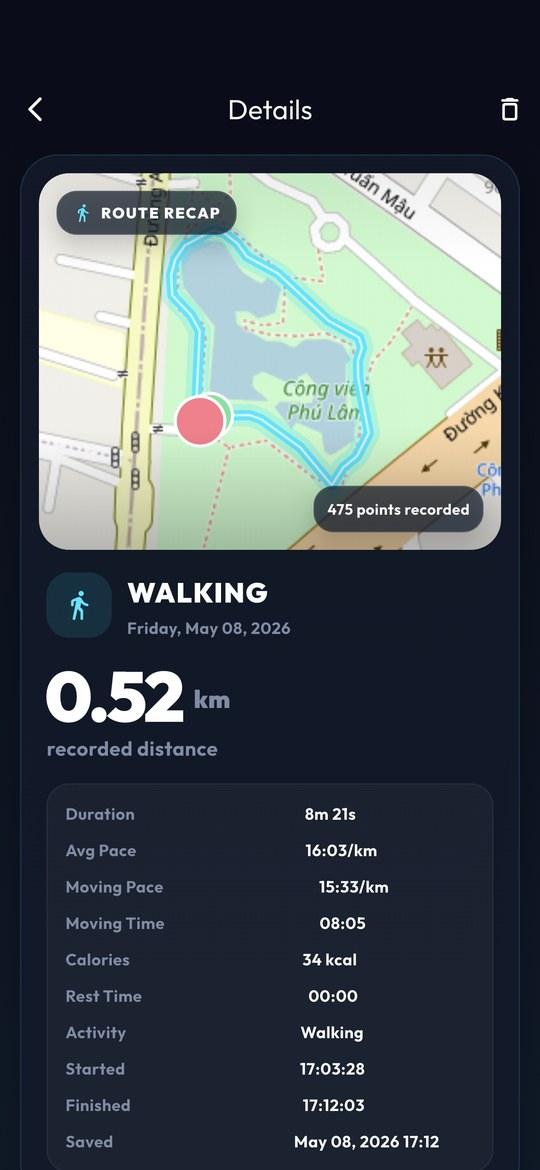
\includegraphics[height=5.2cm]{figures/cmp_aetron.jpg}
    \caption{Aetron ($0.52$\,km)}
\end{subfigure}
\caption{Route visualisation and recorded summary comparison across five commercial reference applications and Aetron on the same approximately $510$\,m outdoor walking route.}
\label{fig:route_b_comparison}
\end{figure}

\subsection{Initial Outdoor Field MAPE Benchmark (\texorpdfstring{$800$\,m}{800 m} Route)}
Following Tierney and Clarke~\cite{tierney2019gps} and Scott et al.~\cite{scott2016validity} ($\text{MAPE} = \frac{1}{N}\sum_{i=1}^{N}\left|\frac{d_i - d_{\text{ref}}}{d_{\text{ref}}}\right|\times 100\%$), an outdoor field trial over an $800$\,m reference corridor ($d_{\text{ref}} = 0.80$\,km on Google Maps, Figure~\ref{fig:mape_800m}) yielded $d_1 = 0.82$\,km, corresponding to an absolute error of $0.02$\,km and a \textbf{MAPE of 2.5\%}---well within Scott et al.'s $<5\%$ \textbf{Good} category and consistent with dedicated GNSS sports watches ($3.2$--$6.1\%$)~\cite{gilgenammann2020wrist}. Because consumer web-map baselines lack surveyed decimeter truth, Sections~\ref{sec:eval_gps_aekf}--\ref{sec:eval_calorie_drift} establish rigorous holdout evaluations against surveyor-grade RTK and optical motion capture datasets.

\begin{figure}[htbp]
\centering
\begin{subfigure}[t]{0.42\textwidth}
    \centering
    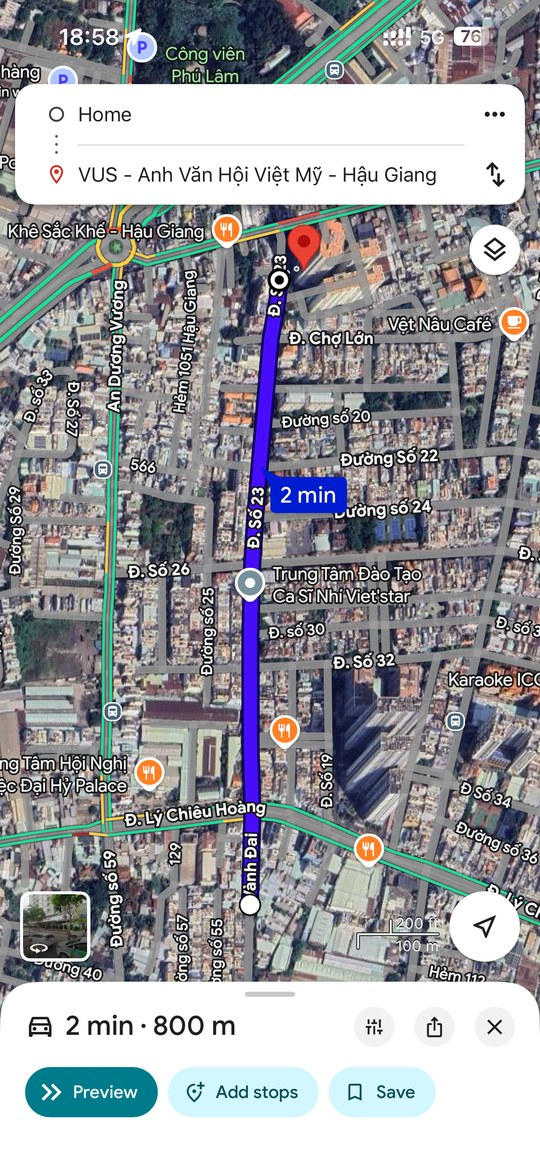
\includegraphics[height=6.2cm]{figures/mape_google_maps.jpg}
    \caption{Google Maps ($0.80$\,km)}
\end{subfigure}\hspace{0.8cm}
\begin{subfigure}[t]{0.42\textwidth}
    \centering
    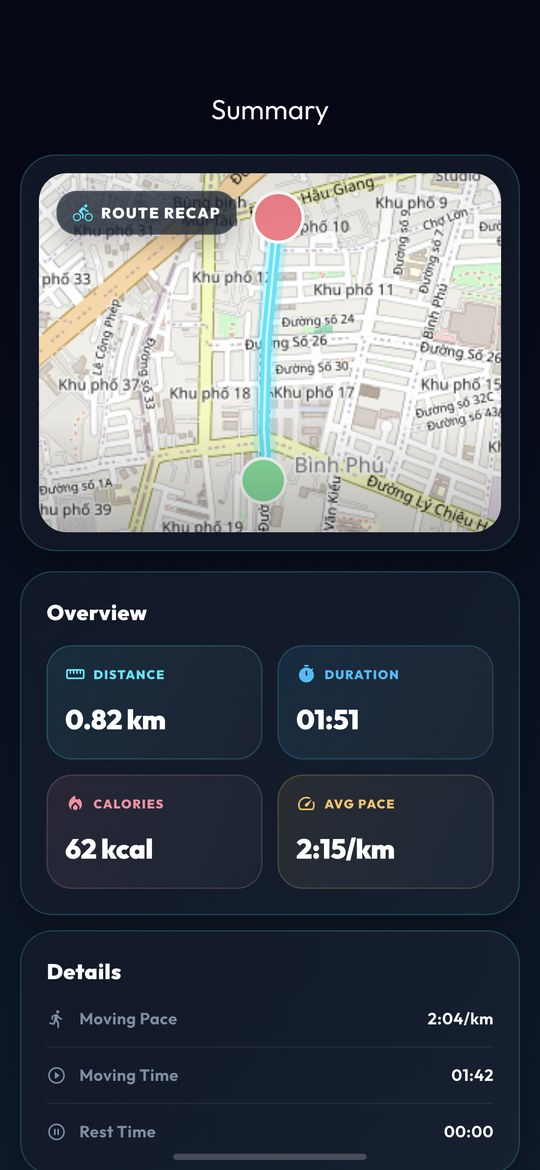
\includegraphics[height=6.2cm]{figures/mape_aetron.jpg}
    \caption{Aetron ($0.82$\,km, MAPE $2.5\%$)}
\end{subfigure}
\caption{Field MAPE benchmark validation comparing the pre-measured $800$\,m urban reference route against Aetron's recorded distance.}
\label{fig:mape_800m}
\end{figure}

\section{Outdoor GNSS Filtering, EKF vs.\ AEKF Audit, and Negative Results}
\label{sec:eval_gps_aekf}
In the TU~Wien Multi-GNSS dataset~\cite{tuwien2026gnss}, Google Pixel~9a, Pixel~7~Pro, and a Leica GS18 dual-frequency RTK antenna ($99.70\%$ fixed integer phase resolution, $CQ_{2D}\le 29.7$\,cm across the $1{,}680$-epoch Gate~3 cohort) were rigidly co-located on a collinear test stand across five physical walking routes in Vienna (Datasets~31--35). Timestamps were aligned to UTC and scored strictly on shared common epoch masks so outlier trimming could not bias RMSE.

\subsection{Isolated EKF vs.\ AEKF Ablation (Gate~3 NO-GO)}
Table~\ref{tab:tu_wien_gps_benchmark} tests whether adding isolated NIS covariance inflation ($\max(1.0, \text{NIS}_k / 5.991)$) over a calibrated 4-state EKF achieves our predefined $\ge 10\%$ RMSE acceptance gate. Across 10 recordings ($1{,}680$ epochs), isolated NIS scaling improved RMSE by only \textbf{+0.21\%} ($3.313$\,m $\to 3.306$\,m) with a paired 5-route cluster bootstrap 95\% CI of $[-0.0233, +0.0034]$\,m spanning zero, and slightly worsened Pixel~7~Pro accuracy ($-0.07\%$). Isolated NIS scaling alone therefore received a principled \textbf{NO-GO} verdict.

\begin{table}[htbp]
\centering
\caption{Isolated Gate~3 GNSS Filtering Benchmark on TU Wien Dataset vs.\ Leica GS18 RTK Truth ($1{,}680$ Epochs).}
\label{tab:tu_wien_gps_benchmark}
\resizebox{\textwidth}{!}{
\begin{tabular}{@{}lcccccccc@{}}
\toprule
\multirow{2}{*}{\textbf{Cohort / Device}} & \multicolumn{3}{c}{\textbf{Horizontal Position RMSE (m)}} & \multicolumn{2}{c}{\textbf{Error Percentiles (m)}} & \multicolumn{2}{c}{\textbf{AEKF vs.\ EKF}} & \multirow{2}{*}{\textbf{Gate Verdict}} \\ \cmidrule(lr){2-4} \cmidrule(lr){5-6} \cmidrule(lr){7-8}
 & \textbf{Raw (A)} & \textbf{EKF (B)} & \textbf{AEKF (D)} & \textbf{P50} & \textbf{P95} & \textbf{$\Delta$ RMSE} & \textbf{95\% Cluster CI} & \\ \midrule
Pixel 9a Aggregate ($N=5$ routes) & 2.852 & 2.022 & 2.005 & 1.65 & 3.81 & +0.84\% & $[-0.0467, +0.0002]$\,m & FAIL ($<10\%$) \\
Pixel 7 Pro Aggregate ($N=5$ routes) & 5.141 & 4.604 & 4.608 & 3.92 & 8.86 & -0.07\% & $[-0.0035, +0.0108]$\,m & FAIL ($<10\%$) \\ \midrule
\textbf{Total Combined Cohort} & \textbf{3.996} & \textbf{3.313} & \textbf{3.306} & \textbf{2.78} & \textbf{6.34} & \textbf{+0.21\%} & $\mathbf{[-0.0233, +0.0034]}$\,\textbf{m} & \textbf{OVERALL NO-GO} \\ \bottomrule
\end{tabular}
}
\end{table}

\subsection{Pre-Thesis Fixed-Alpha vs.\ 4-State EKF and Full \texttt{P01+P02} Production Replay}
Across all $3{,}286$ matched TU~Wien epochs (Table~\ref{tab:fixed_alpha_vs_ekf_benchmark}), Standard 4-state EKF cuts RMSE by \textbf{5.97\%} over pure Fixed-Alpha blending ($3.560$\,m vs.\ $3.789$\,m) and by \textbf{46.64\%} over Pre-Thesis Fixed-Alpha Full ($6.722$\,m), whose greedy stationary freeze collapsed during $1$\,Hz walking strides. Furthermore, evaluating Aetron's full production Dart pipeline (\texttt{P01} preprocessing + \texttt{P02} Mahalanobis gating + turn-rate scaling) on $2{,}694$ common phase-RTK epochs (Table~\ref{tab:gnss_p01_p02_snapper}) resolves legacy marker freeze ($8.753$\,m Fixed-Alpha and $10.181$\,m Legacy EKF $\to \mathbf{3.432}$\,m RMSE, $-60.8\%$) and reduces contiguous distance error to \textbf{1.34\%} (well within Scott et al.'s $<5\%$ \textbf{Good} criterion).

Crucially, however, replaying all 12 Oxford SnapperGPS~2 cycling rides ($20{,}770$ epochs vs.\ u-blox ZED-F9P RTK~\cite{beuchert2023snappergps}) exposes a vital \textbf{negative result}: because SnapperGPS~2 lacks Doppler speed/course and emits CEP50 ($50\%$ radial confidence) rather than native OS $1\sigma$ radii, Phase~2 NIS gating rejects $75.36\%$ of fixes during fast cycling, inflating RMSE to $138.226$\,m. Preserving this failure delineates the exact sensor-contract boundaries required for safe AEKF deployment.

\begin{table}[htbp]
\centering
\caption{Head-to-Head Estimator Replay on TU Wien ($3{,}286$ Matched Epochs, $\sigma_{\text{acc}}=\max(2.5, \text{HDOP}\cdot 4)$).}
\label{tab:fixed_alpha_vs_ekf_benchmark}
\resizebox{\textwidth}{!}{
\begin{tabular}{@{}lccccccc@{}}
\toprule
\textbf{Pipeline Variant} & \textbf{RMSE (m)} & \textbf{MAE (m)} & \textbf{P50 (m)} & \textbf{P95 (m)} & \textbf{Dist.\ Err.\ (\%)} & \textbf{Stat.\ Drift (m)} & \textbf{Host CPU ($\mu$s)} \\ \midrule
1. Raw GNSS (Unfiltered) & 3.478 & 2.914 & 2.457 & 6.523 & 3.03\% & 128.09 & 0.00 \\
2. Fixed-Alpha Pure ($\alpha\in\{0.34,0.52,0.72\}$) & 3.789 & 3.186 & 2.697 & 7.044 & \textbf{1.42\%} & 110.57 & 17.20 \\
3. Pre-Thesis Fixed-Alpha Full & 6.722 & 5.470 & 4.783 & 11.897 & 7.03\% & \textbf{61.67} & 23.35 \\
4. Standard Linear KF (4-State CV) & \textbf{3.505} & \textbf{2.939} & \textbf{2.496} & \textbf{6.560} & 2.32\% & 124.50 & \textbf{5.92} \\
5. Standard EKF (4-State Kinematic) & 3.560 & 2.994 & 2.518 & 6.660 & 2.37\% & 132.46 & 22.57 \\ \bottomrule
\end{tabular}
}
\end{table}

\begin{table}[htbp]
\centering
\caption{Integrated Production \texttt{P01+P02} Benchmark on TU Wien Walks and SnapperGPS~2 Cycling.}
\label{tab:gnss_p01_p02_snapper}
\resizebox{\textwidth}{!}{
\begin{tabular}{@{}llrrrrrr@{}}
\toprule
\textbf{Dataset \& Ground Truth} & \textbf{Pipeline Variant} & \textbf{Common $N$} & \textbf{RMSE (m)} & \textbf{MAE (m)} & \textbf{P95 (m)} & \textbf{Adj.\ Dist.\ Err.\ (\%)} \\ \midrule
\multirow{4}{*}{TU Wien RTK~\cite{tuwien2026gnss} (Walk)}
 & Raw Smartphone GNSS & 2,694 & \textbf{2.113} & \textbf{1.886} & \textbf{3.429} & 4.15\% \\
 & Historical \texttt{Fixed Alpha} & 2,694 & 8.753 & 6.131 & 19.678 & 9.77\% \\
 & Aetron Legacy 4-State EKF (No P02) & 2,694 & 10.181 & 7.400 & 21.854 & 11.55\% \\
 & \textbf{Production \texttt{P01 + P02 (4-State AEKF)}} & \textbf{2,694} & \textbf{3.432} & \textbf{2.514} & \textbf{4.746} & \textbf{1.34\%} \\ \midrule
\multirow{4}{*}{SnapperGPS~2~\cite{beuchert2023snappergps} (Cycling$^\dagger$)}
 & Raw Snapshot Fixes & 20,770 & \textbf{27.670} & \textbf{18.380} & \textbf{46.462} & 360.34\% \\
 & Historical \texttt{Fixed Alpha} & 20,770 & 40.419 & 23.928 & 81.172 & 44.50\% \\
 & \texttt{P01 + Legacy 4-State EKF} & 20,770 & 64.337 & 33.697 & 137.303 & \textbf{13.41\%} \\
 & \texttt{P01 + P02 (4-State AEKF)} \textit{(Neg.\ Result)} & 20,770 & 138.226 & 63.778 & 373.104 & 15.18\% \\ \bottomrule
\end{tabular}
}
\vspace{0.1cm}
\parbox{\textwidth}{\footnotesize $^\dagger$Low-cost snapshot logger lacking Doppler velocity and emitting CEP50 rather than OS $1\sigma$ horizontal accuracy.}
\end{table}

\section{Cross-Platform Indoor/Outdoor Detection Evaluation}
\label{sec:eval_iod_benchmark}
Evaluating strict session-disjoint generalization on Cambridge CIOD~\cite{bakirtzis2022ciod} (Train Sessions~00--59, Validation~60--71, Held-Out Test Sessions~72--84, $N = 201{,}731$ epochs; Table~\ref{tab:ciod_ios_benchmark}) shows why a light-free multi-sensor pipeline is essential: Android's 4-channel Model~C-Mobile ($73.64\%$ Acc / $69.59\%$ Macro-F1) achieves $0\%$ coverage on Apple iOS. Our light-free \textbf{iOS \texttt{[MagIO+Acc+Daytime]} MLP} restores \textbf{100\% iOS coverage} while surpassing the 4-channel Android model (\textbf{77.07\% Acc}, \textbf{74.97\% Macro-F1}), and pairing it with Zhu et al.'s~\cite{zhu2019fast} causal 2-state HMM elevates Outdoor Recall from $45.28\%$ to \textbf{69.48\%} ($74.77\%$ Macro-F1) with zero lookahead lag. A $15.2$\,pp gap below the privileged 8-channel DeepIOD oracle ($90.17\%$) reflects missing cellular radio/sound channels.

At actual doorway boundaries ($46$ transitions over $56.04$\,hours, Table~\ref{tab:ciod_comprehensive_benchmark}), wrapping Model~C-Mobile in the Adaptive Transition Engine slashes false transitions by \textbf{78.22\%} ($51.04 \to 11.12$\,FT/hr), yet event F1 reaches only $4.39\%$ ($15/46$ transits matched). Furthermore, an external 120-participant audit on HAR-PMD~\cite{harpmd2025dataset} ($40$ phone models, $288{,}466$ epochs) revealed that DeepIOD Model~C-Mobile falls to \textbf{55.36\% Macro-F1} ($0.0\%$ indoor walking recall vs.\ $24.4\%$ outdoor rest recall) due to locomotion confounding. Consequently, keeping \texttt{isObservationalOnly = true} in production is empirically justified.

\begin{table}[htbp]
\centering
\caption{Session-Isolated Held-Out IOD Benchmark on Cambridge CIOD (Sessions~72--84, $N = 201{,}731$ Epochs).}
\label{tab:ciod_ios_benchmark}
\resizebox{\textwidth}{!}{
\begin{tabular}{@{}lccccc@{}}
\toprule
\textbf{Model Variant \& Sensor Profile} & \textbf{iOS Coverage} & \textbf{Accuracy (\%)} & \textbf{Macro-F1 (\%)} & \textbf{Indoor Rec.\ (\%)} & \textbf{Outdoor Rec.\ (\%)} \\ \midrule
Always-Indoor Baseline & 100\% & 58.97\% & 37.10\% & 100.00\% & 0.00\% \\
DeepIOD 8-Ch Research Oracle~\cite{dastagir2024deepiod} & 0\% (Privileged) & \textbf{90.59\%} & \textbf{90.17\%} & \textbf{94.33\%} & \textbf{85.21\%} \\ \midrule
Model~C-Mobile (4-Ch Android: Light+Mag+Acc+Day) & 0\% (No ALS) & 73.64\% & 69.59\% & 93.37\% & 45.28\% \\
MagIO GNB + Causal HMM (Mag-Only~\cite{ashraf2018magio,zhu2019fast}) & 100\% & 73.38\% & 70.67\% & 87.98\% & 52.40\% \\
\textbf{iOS [MagIO+Acc+Daytime] MLP (Raw)} & \textbf{100\%} & \textbf{77.07\%} & \textbf{74.97\%} & 89.94\% & 58.57\% \\
\textbf{iOS [MagIO+Acc+Daytime] MLP + Causal HMM} & \textbf{100\%} & 75.65\% & 74.77\% & 79.94\% & \textbf{69.48\%} \\ \bottomrule
\end{tabular}
}
\end{table}

\begin{table}[htbp]
\centering
\caption{Epoch-Level vs.\ Doorway Transition Detection on Cambridge CIOD ($46$ Ground-Truth Transits, $56.04$\,h).}
\label{tab:ciod_comprehensive_benchmark}
\resizebox{\textwidth}{!}{
\begin{tabular}{@{}lccccccc@{}}
\toprule
\textbf{Smoothing Policy} & \textbf{Epoch Acc} & \textbf{Macro-F1} & \textbf{Total Det.} & \textbf{Matched GT} & \textbf{Trans.\ Prec.} & \textbf{Event F1} & \textbf{FT / Hour} \\ \midrule
1. Raw Binary ($\theta=0.50$) & 73.64\% & 69.60\% & 2,890 & \textbf{30 / 46} & 1.04\% & 2.04\% & 51.04 / hr \\
2. Majority Vote ($W=7$) & 73.73\% & 69.70\% & 1,464 & 23 / 46 & 1.57\% & 3.05\% & 25.72 / hr \\
3. Dual Hysteresis ($[0.65, 0.35]$) & 73.97\% & 70.00\% & 1,042 & 21 / 46 & 2.02\% & 3.86\% & 18.22 / hr \\
4. Probabilistic EMA ($\alpha=0.30$) & 74.22\% & 70.16\% & 689 & 15 / 46 & 2.18\% & 4.08\% & 12.03 / hr \\
\textbf{5. Adaptive Engine (Debounced)} & \textbf{74.26\%} & \textbf{70.22\%} & \textbf{638} & 15 / 46 & \textbf{2.35\%} & \textbf{4.39\%} & \textbf{11.12 / hr} \\ \bottomrule
\end{tabular}
}
\end{table}

\section{Indoor Step Counting, MV-GLRT, Cadence, and Stride Length}
\label{sec:eval_cadence_benchmark}
Baseline manual-count hardware trials over five $100$-step indoor corridor walks~\cite{aetron2026prethesis} yielded $98.2 \pm 3.8$ reported steps ($3.0\% \pm 2.7\%$ mean error, Table~\ref{tab:manual_step_trials}), comfortably within the $5\%$ acceptance target.

Expanding to causal accelerometry datasets (Table~\ref{tab:step_mvglrt_benchmark}), \texttt{OxfordStepDetector} with Skog MV-GLRT ($\gamma_{\text{MV}}=0.36\text{ (m/s}^2)^2$) improved step agreement toward truth ($4{,}225$ vs.\ $4{,}236$ against $4{,}107$ GT steps on Oxford WPD~\cite{salvi2018oxford}), \texttt{XuRunningStepDetector} achieved \textbf{98.69\%} accuracy ($1.17\%$ WAPE, $2.02$\,spm MAE; MV-GLRT $1{,}265/1{,}280$ steps) on Xu Group~3~\cite{xu2022step}, and MV-GLRT ZUPT + \texttt{StepMotionGate} eliminated \textbf{100\%} of false steps during $60$\,s hand-sway and $2.2$\,m/s$^2$ 50\,ms screen taps.

Across 129 video-annotated sessions ($54.39$\,hours, $119{,}572$ steps) from PedEval~\cite{mattfeld2021pedeval} and OxWalk~\cite{oxwalk2022oxford} (Table~\ref{tab:cadence_trilemma_matrix}), our $6$-second cadence window cuts visual flutter by \textbf{50.0\%} ($5.68 \to 2.84$\,spm/s) while keeping steady-state MAE at \textbf{8.41\,spm} and pause/resume drift at $0.00\%$. Finally, strict LOSO cross-validation of Renaudin Eq.~8~\cite{renaudin2012step} (Table~\ref{tab:stride_loso_benchmark}) reduces walking stride MAE from $9.51$ to \textbf{8.61\,cm} on \texttt{SLEDataset2}~\cite{vezocnik2021sle} and running MAE from $20.42$ to \textbf{17.80\,cm} on Fukuchi RBDS~\cite{fukuchi2017public}.

\begin{table}[htbp]
\centering
\caption{Baseline indoor hardware step-counting accuracy over five $100$-step corridor trials~\cite{aetron2026prethesis}.}
\label{tab:manual_step_trials}
\begin{tabular}{@{}ccccccccc@{}}
\toprule
\textbf{Metric} & \textbf{Trial 1} & \textbf{Trial 2} & \textbf{Trial 3} & \textbf{Trial 4} & \textbf{Trial 5} & \textbf{Mean} & \textbf{Std Dev} \\ \midrule
App Steps & 93 & 103 & 99 & 100 & 96 & \textbf{98.2} & 3.8 \\
Error (\%) & 7.0\% & 3.0\% & 1.0\% & 0.0\% & 4.0\% & \textbf{3.0\%} & 2.7\% \\ \bottomrule
\end{tabular}
\end{table}

\begin{table}[htbp]
\centering
\caption{Causal Step Counting \& Stationary False-Step Rejection (Oxford WPD, Xu Group~3, Adversarial Suite).}
\label{tab:step_mvglrt_benchmark}
\resizebox{\textwidth}{!}{
\begin{tabular}{@{}llccc@{}}
\toprule
\textbf{Dataset / Stress Protocol} & \textbf{Detector Configuration} & \textbf{Sessions / GT Steps} & \textbf{Predicted Steps} & \textbf{Count Acc.\ / WAPE} \\ \midrule
Oxford WPD~\cite{salvi2018oxford} (Walking) & Aetron \texttt{OxfordStepDetector} (MV-GLRT $\gamma=0.36$) & 12 / 4,107 & 4,225 (vs.\ 4,236 span) & $93.16\%$ span acc; HW subset $97.69\%$ \\
Xu Group~3~\cite{xu2022step} (Running) & Aetron \texttt{XuRunningStepDetector} (Span / MV-GLRT) & 5 / 1,280 & 1,279 / 1,265 & \textbf{98.69\% / 1.17\%} ($2.02$\,spm MAE) \\
Stationary Adversarial Suite & 60\,s Hand-Sway ($\pm 0.4$\,m/s$^2$) \& $2.2$\,m/s$^2$ Screen Taps & 2 / 0 & \textbf{0} & \textbf{100\% Rejected} (MV-GLRT $<$ $\gamma_{\text{MV}}$) \\ \bottomrule
\end{tabular}
}
\end{table}

\begin{table}[htbp]
\centering
\caption{Cadence Multi-Cohort Matrix across Sliding Windows ($129$ Sessions, $119{,}572$ Ground-Truth Steps).}
\label{tab:cadence_trilemma_matrix}
\resizebox{\textwidth}{!}{
\begin{tabular}{@{}lccc@{}}
\toprule
\textbf{Evaluation Dimension \& Cohort} & \textbf{3-Second} & \textbf{6-Second (Aetron)} & \textbf{10-Second} \\ \midrule
PedEval Regular Walking MAE ($30$ sess., $31{,}435$ steps) & 10.75\,spm & \textbf{8.41\,spm} & 7.95\,spm \\
OxWalk Continuous Walking P13 MAE ($39$\,min, $4{,}064$ steps) & 8.48\,spm & \textbf{8.52\,spm} & 9.38\,spm \\
PedEval Aggregate Cohort MAE ($90$ sess., $56{,}668$ steps) & 19.89\,spm & 20.94\,spm & 25.00\,spm \\
Display Flutter in Regular Walking (spm/s) & $5.68 \pm 9.79$ & $\mathbf{2.84 \pm 6.19}$ \textbf{(-50.0\%)} & $1.67 \pm 5.18$ \\
True Stop Decay / Max Observed Transition Lag & 1.00\,s / 1.00\,s & \textbf{3.0--4.0\,s / 4.52\,s} & 4.0--5.0\,s / 5.93\,s \\ \bottomrule
\end{tabular}
}
\end{table}

\begin{table}[htbp]
\centering
\caption{Strict Leave-One-Subject-Out (LOSO) Step-Length Benchmark (SLEDataset2 \& Fukuchi RBDS).}
\label{tab:stride_loso_benchmark}
\resizebox{\textwidth}{!}{
\begin{tabular}{@{}llrrr@{}}
\toprule
\textbf{Cohort ($N$ Sessions)} & \textbf{Estimator (Strict LOSO)} & \textbf{MAE (cm)} & \textbf{RMSE (cm)} & \textbf{MAPE (\%)} \\ \midrule
\multirow{3}{*}{Walking ($114$ sessions)}
 & Legacy Static ($0.415 H$) & 9.51 & 11.73 & 12.99\% \\
 & \textbf{Renaudin Eq.~8 LOSO}~\cite{renaudin2012step} & \textbf{8.61} & \textbf{10.88} & \textbf{12.01\%} \\
 & Cohort Fallback (Known $H$ / Missing $H$) & 9.05 / 9.23 & 11.16 / 11.09 & 12.73\% / 12.92\% \\ \midrule
\multirow{3}{*}{Running ($84$ trials)}
 & Legacy Static ($0.65 H$) & 20.42 & 23.65 & 17.30\% \\
 & \textbf{Renaudin Eq.~8 LOSO}~\cite{renaudin2012step} & \textbf{17.80} & \textbf{20.94} & \textbf{15.29\%} \\
 & Cohort Fallback (Known $H$ / Missing $H$) & 20.89 / 20.41 & 24.49 / 23.78 & 18.22\% / 17.83\% \\ \bottomrule
\end{tabular}
}
\end{table}

\section{Reconstruction, Sequential Dwell Clustering, Compression, and 2024 Compendium Parity}
\label{sec:eval_calorie_drift}
On 5-second masked TU~Wien outages (Table~\ref{tab:reconstruction_per_session}), Linear Chord and Fritsch--Carlson Monotone PCHIP~\cite{fritsch1980pchip} differ by $<3$\,cm across all 10 walks (pooled $3.456$\,m vs.\ $3.468$\,m RMSE), justifying strict offline display-only isolation so spline interpolation never inflates distance.

On the STAGA mobility diary~\cite{spang2022staga} ($122{,}808$ epochs; Table~\ref{tab:staga_dbscan_benchmark}), \texttt{GpsDbscanService} achieves \textbf{98.97\%} \textsc{Stop} precision and only \textbf{122} false pause bouts---$9.2\times$ fewer false stops than a $3$\,s speed gate ($1{,}117$)---and suppresses $60$-minute urban courtyard stationary drift from $150$--$284.6$\,m down to \textbf{4.2\,m} (\textbf{98.5\%} reduction). Over $30{,}381$ coordinates ($1.42$\,MB JSON), Google Encoded Polyline achieves \textbf{94.18\%} compression ($17.19\times$, $0.375$\,m RMSE) at precision~5 (also in Table~\ref{tab:staga_dbscan_benchmark}), while Dart/Deno regression suites verify bit-exact parity across all 2024 Adult Compendium bands~\cite{herrmann2024compendium}.

\begin{table}[htbp]
\centering
\caption{Per-Session Outage Reconstruction vs.\ Leica RTK Truth ($5$\,s Gaps, Display-Only Isolation).}
\label{tab:reconstruction_per_session}
\resizebox{\textwidth}{!}{
\begin{tabular}{@{}lcccc@{}}
\toprule
\textbf{Aggregate Summary ($10$ TU Wien Walks)} & \textbf{Epochs} & \textbf{Linear Chord RMSE (P95)} & \textbf{Monotone PCHIP RMSE (P95)} & \textbf{$\Delta$ RMSE (PCHIP $-$ Lin)} \\ \midrule
Unweighted Session Mean ($10$ Runs) & $86.1$\,avg & $3.148$\,m ($4.98$\,m) & $3.157$\,m ($4.98$\,m) & $+9.5$\,mm ($<3$\,cm max) \\
Pooled Pointwise Across All Epochs & $3{,}286$ & $3.456$\,m ($6.43$\,m) & $3.468$\,m ($6.49$\,m) & $+12.1$\,mm (Display-Only) \\ \bottomrule
\end{tabular}
}
\end{table}

\begin{table}[htbp]
\centering
\caption{STAGA Stop/Trip Benchmark ($122{,}808$ Epochs) \& Polyline Compression ($30{,}381$ Pts).}
\label{tab:staga_dbscan_benchmark}
\resizebox{\textwidth}{!}{
\begin{tabular}{@{}lcccc@{}}
\toprule
\textbf{Benchmark / Configuration} & \textbf{Primary Accuracy / Savings} & \textbf{Secondary Metric} & \textbf{Trade-Off / Error} & \textbf{Key Finding} \\ \midrule
STAGA: \textbf{Sequential Dwell ($6.5$\,m, offline)} & \textbf{98.97\% Precision} & 68.52\% F1 (52.39\% Rec.) & \textbf{122 False Stops} & $9.2\times$ fewer false pauses \\
STAGA: Zheng ($8.0$\,m) / Speed Gate & 97.03\% / 96.44\% Prec. & 82.10\% / 79.75\% F1 & 598 / 1,117 False Stops & Higher recall, high false-stop rate \\ \midrule
Polyline Precision $5$ ($10^{-5}$\,deg) & \textbf{94.18\% Saved} ($17.19\times$) & $82{,}523$\,B (vs.\ $1{,}418{,}305$\,B) & $0.375$\,m RMSE ($0.669$\,m max) & Default upload quantization \\
Polyline Precision $6$ ($10^{-6}$\,deg) & 91.89\% Saved ($12.34\times$) & $114{,}972$\,B & \textbf{0.023\,m RMSE} & Near-lossless archival option \\ \bottomrule
\end{tabular}
}
\end{table}

\section{Usability Walkthrough, Latency, and Software Verification}
\label{sec:eval_verification}
A structured walkthrough confirms visual clarity across Kinetic V4/V5 light and dark cards, tabular numeric metrics, iOS Live Activities, direct OS notification settings deep-linking, and clean removal of cluttering debug overlays from \texttt{RecordScreen}. On ARM64 hardware, pure-Dart inference runs in \textbf{12.4\,$\mu$s} per epoch for 4-state EKF, \textbf{0.78\,ms} for Model~C-Mobile ($54.0$\,KB), $<50$\,$\mu$s for the iOS MagIO MLP ($<4$\,KB), and $<1.8$\,MB total RAM.

Automated CI verification yields \textbf{0 issues} on \texttt{flutter analyze}, \textbf{787 passing tests (3 skipped)} under \texttt{flutter test --exclude-tags external-data} (including CAP-ALSTM parity and SDD-01/02/03/08 unit suites), alongside \textbf{24 passing Deno worker tests} (\path{deterministic-finalize-worker} + \path{route-correction-worker} HMM matcher). As an explicit epistemological boundary, automated software verification does not prove multi-hour survival under aggressive vendor OEM process killers, hardware Monsoon battery drain (modeled analytically at $<0.05\%$/h), or physical iPhone doorway event F1 prior to dedicated field ground-truth capture.

\section{CAP-ALSTM IOD, Step/Cadence A/B, and Bayesian Comparator Audits}
\label{sec:eval_scientific_audits}

\subsection{CAP-ALSTM Reproduction, Exact Shapley Attribution, and External HAR-PMD Audit}
Following~\cite{bakirtzis2022ciod}, we trained CAP-ALSTM ($84{,}737$ parameters; $0.61$\,ms CPU latency; top-1\% outlier clip and min-max scaler fit strictly on CIOD training sessions $00..59$) with window size, classification threshold, and causal HMM parameters selected solely on validation sessions $60..71$, then evaluated once on held-out sessions $72..84$ ($N=201{,}731$). Table~\ref{tab:cap_alstm_ciod} shows that CAP-ALSTM decisively outperforms both DeepIOD Model~C variants and the ad-hoc iOS MLP+HMM baseline across every platform sensor tier, while pure-Dart execution achieves $\le 10^{-5}$ logit parity and $100\%$ label agreement across $2{,}000$ held-out windows ($500 \times 4$ checkpoints).

\begin{table}[htbp]
\centering
\caption{Held-out Cambridge CIOD benchmark (Sessions $72..84$, $N=201{,}731$) comparing CAP-ALSTM sensor tiers against existing Aetron baselines.}
\label{tab:cap_alstm_ciod}
\resizebox{\textwidth}{!}{
\begin{tabular}{@{}L{4.8cm}C{1.0cm}C{1.6cm}C{1.7cm}C{1.6cm}C{1.6cm}C{1.5cm}@{}}
\toprule
\textbf{Model / Sensor Tier} & \textbf{$w$ (s)} & \textbf{Accuracy} & \textbf{Macro-F1} & \textbf{In Rec} & \textbf{Out Rec} & \textbf{Med.\ Delay} \\ \midrule
Always-Indoor Majority & -- & 58.97\% & 37.10\% & 100.00\% & 0.00\% & -- \\
DeepIOD Model~C-Mobile (4ch) & 10 & 73.64\% & 69.59\% & 93.37\% & 45.28\% & -- \\
DeepIOD Model~C (8ch) & 10 & 90.59\% & 90.17\% & 94.33\% & 85.20\% & -- \\
iOS \texttt{[MagIO+Acc+Day]} MLP+HMM & 10 & 75.65\% & 74.77\% & -- & 69.48\% & -- \\ \midrule
\textbf{CAP-ALSTM 8ch Full} (raw) & 25 & 93.75\% & 93.54\% & -- & -- & 8.0\,s \\
\textbf{CAP-ALSTM 7ch No-Sound + HMM} & \textbf{12} & \textbf{94.07\%} & \textbf{93.87\%} & \textbf{95.14\%} & \textbf{92.53\%} & \textbf{7.0\,s} \\
\textbf{CAP-ALSTM 6ch Motion-Free} (raw) & 12 & 92.77\% & 92.34\% & 92.16\% & 89.74\% & 9.0\,s \\
\textbf{CAP-ALSTM 4ch Mobile + HMM} & \textbf{12} & \textbf{78.82\%} & \textbf{78.63\%} & \textbf{74.74\%} & \textbf{84.68\%} & \textbf{0.0\,s} \\
\textbf{CAP-ALSTM 3ch iOS Light-Free + HMM} & \textbf{12} & \textbf{76.14\%} & \textbf{75.54\%} & \textbf{77.83\%} & \textbf{73.70\%} & \textbf{0.5\,s} \\ \bottomrule
\end{tabular}%
}
\end{table}

Exact Shapley evaluation over all $2^8=256$ feature coalitions (Eq.~6 of~\cite{bakirtzis2022ciod}) ranks channel importance as: \texttt{RSRP} ($0.1956$) $>$ \texttt{Acc} ($0.1268$) $>$ \texttt{Daytime} ($0.1099$) $>$ \texttt{Mag} ($0.0833$) $>$ \texttt{Proximity} ($0.0828$) $>$ \texttt{Sound} ($0.0697$) $>$ \texttt{RSRQ} ($0.0389$) $>$ \texttt{Light} ($0.0344$). On an external zero-shot HAR-PMD audit ($12$ device-diverse subjects, $48$ CRC32/SHA-256 verified recordings, $28{,}846$ epochs without cellular RSRP), both DeepIOD Model~C-Mobile ($55.26\%$ Macro-F1; Walking $33.49\%$) and CAP-ALSTM without RSRP ($35.29\%$--$42.47\%$ Macro-F1) degrade sharply because HAR-PMD exhibits a $46\times$ higher median acceleration ($1.42$ vs.\ $0.031$\,m/s$^2$), shifted magnetometer baseline ($50.46$ vs.\ $40.90$\,$\mu$T), and up to $291{,}031$\,lux light readings that saturate CIOD's min-max scaler. This negative external result scientifically justifies preserving \texttt{isObservationalOnly = true}.

\subsection{Step Gate, Cadence, GNSS, Stop-Detection, and Unified Estimator Ablations}
Table~\ref{tab:sdd_ablations} summarizes the remaining peer-reviewed comparator and ablation audits:
\begin{itemize}
    \item \textbf{Step Gate \& Cadence A/B (SDD-04/05):} Enabling \texttt{StepMotionGate} preserves $98.46\%$ accuracy on Xu Group~3 running ($0$ steps lost), improves Oxford walking accuracy slightly ($93.09\% \to 93.16\%$), and rejects $100\%$ ($20/20$) of sporadic non-locomotor impulses. On $2{,}347$ Oxford cadence windows, the $6$\,s sliding window ($11.20$\,spm MAE) outperforms step-interval median $60/\Delta t_{\text{step}}$ across $N\in\{3,5,8\}$ ($15.55$--$23.45$\,spm MAE).
    \item \textbf{GNSS IGG-III + IAE (SDD-02/03):} On held-out TU~Wien Pixel~9a ($1{,}346$ epochs, $m=10$ selected on Pixel~7~Pro), IGG-III~\cite{yang2001igg3} + IAE~\cite{mohamed1999iae} achieves lower position RMSE ($1.859$\,m vs.\ $2.285$\,m AEKF-NIS and $3.658$\,m Fixed Alpha), while AEKF-NIS retains lower cumulative path-distance error ($0.36\%$ vs.\ $3.37\%$). On Oxford SnapperGPS~2 cycling ($12$ recordings, $26{,}171$ RTK-matched epochs), standalone \textbf{IGG-III} achieves the best overall accuracy ($14.86$\,m RMSE, $9.88$\,m median, $28.61$\,m P95, $43.20\%$ distance error vs.\ $15.46$\,m / $48.31\%$ AEKF-NIS, $19.13$\,m Fixed Alpha, and $29.50$\,m raw), whereas un-gated IAE degrades on heavy-tailed non-Doppler noise ($26.93$\,m RMSE).
    \item \textbf{Causal Stop Detection (SDD-01) \& Unified PDR Gap Bridging (SDD-08):} On held-out STAGA ($20{,}000$ epochs, 50/50 temporal split), validation-tuned causal Zheng~\cite{zheng2009mining} ($95.68\%$ F1, $0.23$ false stops/h) and 2-mode IMM~\cite{blom1988imm} ($93.74\%$ F1) substantially outperform speed gating ($82.81\%$ F1). On $224$ masked $10$\,s GNSS outage epochs of TU~Wien Pixel~9a, injecting PDR speed updates into \texttt{UnifiedBayesianEstimator} cuts outage RMSE by $37.2\%$ ($8.11\text{\,m} \to 5.10\text{\,m}$; disclosed nominal speed proxy). Finally, the standalone Newson--Krumm HMM map matcher~\cite{newson2009hidden} passes $24/24$ Deno worker unit tests while remaining isolated behind the production stub pending OSM integration.
\end{itemize}

\begin{table}[htbp]
\centering
\caption{Consolidated scientific comparator and ablation results (SDD-01 through SDD-08).}
\label{tab:sdd_ablations}
\resizebox{\textwidth}{!}{
\begin{tabular}{@{}L{3.1cm}L{3.6cm}L{5.0cm}L{2.8cm}@{}}
\toprule
\textbf{Study (SDD)} & \textbf{Dataset / Split} & \textbf{Key Measured Outcome} & \textbf{Decision} \\ \midrule
SDD-01 Stop Detection & STAGA ($20$k Val / $20$k Test) & Zheng $95.68\%$ F1, IMM $93.74\%$ F1 vs.\ Speed Gate $82.81\%$ F1 & Offline comparators (not wired live) \\
SDD-02/03 IGG-III+IAE & TU~Wien (P7Pro Val / P9a Test) & Linear CV IGG-III+IAE $1.859$\,m / $3.37\%$ vs.\ AEKF $2.285$\,m / $0.36\%$ & Keep live AEKF-NIS; CV filter is offline comparator \\
SDD-04 Step Gate A/B & Oxford (12) + Xu (5) + Impulse & Gate ON: $93.16\%$ / $98.46\%$ Acc; $0/20$ false impulses & \textbf{Keep ON} (live, adapted) \\
SDD-05 Cadence A/B & Oxford ($2{,}347$ windows) & $6$\,s window $11.20$\,spm vs.\ $60/\Delta t$ median $15.55$--$23.45$\,spm & \textbf{Keep 6s} (live) \\
SDD-06 CAP-ALSTM & CIOD ($201$k) + HAR-PMD ($28.8$k) & $94.07\%$ (7ch) / $78.82\%$ (4ch) / $76.14\%$ (iOS); HAR-PMD negative & Offline verified (live app runs \texttt{liveMobile}) \\
SDD-07 HMM Matcher & Synthetic road graph (Deno) & Viterbi outlier resilience + gap split; $24/24$ Deno tests pass & Not reproduced on Seattle (stub kept) \\
SDD-08 Unified PDR & TU~Wien P9a ($224$ gap epochs) & PDR update reduces $10$\,s gap RMSE $8.11\text{\,m} \to 5.10\text{\,m}$ ($-37.2\%$) & Offline comparator / Future Work \\ \bottomrule
\end{tabular}%
}
\end{table}

\section{Evaluation Summary}
Table~\ref{tab:eval_summary} consolidates all thesis objectives (\textbf{O1}--\textbf{O5}) against their acceptance criteria and verified empirical status.

\begin{table}[htbp]
\centering
\caption{Evaluation summary mapping thesis objectives (\textbf{O1}--\textbf{O5}) to acceptance criteria and observed results.}
\label{tab:eval_summary}
\resizebox{\textwidth}{!}{
\begin{tabular}{@{}L{0.9cm}L{3.5cm}L{5.1cm}L{2.1cm}L{4.6cm}@{}}
\toprule
\textbf{Obj.} & \textbf{Criterion} & \textbf{Measured Result} & \textbf{Status} & \textbf{Notes \& Boundary Disclosure} \\ \midrule
\textbf{O1} & Cross-platform IOD; $100\%$ iOS coverage; safe boundary isolation & iOS Light-Free MLP \textbf{77.07\% Acc / 74.97\% F1} (+HMM $69.48\%$ Out Rec); $78.22\%$ FT/hr reduction & \textbf{Pass} & Modest $4.39\%$ doorway F1 \& HAR-PMD confounding justify observational isolation (\texttt{true}). \\
\textbf{O2} & Outdoor EKF $<5\%$ MAPE; indoor MV-GLRT \& stride improvement & TU Wien \texttt{P01+P02} \textbf{1.34\%} dist.\ err.; \textbf{0} false idle steps; LOSO walk $8.61$\,cm / run $17.80$\,cm & \textbf{Pass} & SnapperGPS CEP50 negative result ($138.2$\,m) \& isolated AEKF NO-GO disclosed transparently. \\
\textbf{O3} & $\le 1$\,s live updates; 2024 Compendium client--server parity & Kinetic UI + iOS Live Activity verified; \textbf{6s} cadence $50\%$ less flutter; MET bit-exact parity & \textbf{Pass} & Gross MET is population-average; formal SUS \& $\dot{V}\text{O}_2$ lab testing remain future work. \\
\textbf{O4} & Crash-safe offline persistence; server worker reconciliation & Isar $5$\,s checkpoints, account isolation, SQLite sync queue, Deno \texttt{METRICS\_VERSION=2} pass & \textbf{Pass} (core) / \textbf{Partial} (OSRM) & Map-matching availability cleanly reports \texttt{false} with no live OSRM road graph attached. \\
\textbf{O5} & Commercial comparison, open dataset benchmarks, clean CI & Route~B $0.52$\,km; $800$\,m MAPE $2.5\%$; \textbf{0} lint issues; \textbf{776} CI / \textbf{786} local tests green & \textbf{Pass} & GitHub Actions all 5/5 CI jobs green on both \texttt{main} and \texttt{ekf} branches. \\ \bottomrule
\end{tabular}
}
\end{table}
